\section{Технологический раздел}

В данном разделе будут рассмотрены 
средства программной 
реализации, описание основных моментов программной реализации и 
методики тестирования созданного программного обеспечения. 

\subsection{Технические средства}

В данном разделе будут описаны технические средства, которые
были использованы в процессе разработки программного обеспечения.

\subsubsection{Язык программирования}

Для разработки был выбран язык программирования C++. Из его достоинств следует
выделить высокую скорость (практически сравнимую с языком C для современных
компиляторов) и широкие возможности, позволяющие достаточно писать достаточно
удобный и выразительный код по сравнению с тем же C, а так же вероятно самое
большое количество удобных сторонних библиотек на все случаи жизни. Также C++
предоставляет громоздкие, но крайне эффективные методы шаблонного
метапрограммирования, позволяющие генерировать очень эффективный код из
неповторяющихся блоков. Из недостатков следует выделить относительную сложность синтаксиса и
большое количество правил языка и нетривиальных моментов в языке, из чего
следует потенциально большое количество скрытых ошибок.

Было выбрано подмножество языка C++11, которое даёт разработчику новые
возможности по написанию более быстрого и понятного кода, большие приятные
нововведения в библиотеку C++ STL, а так же новые конструкции для избавления от
некоторых ошибок.

В качестве альтернатив рассматривались некоторые , скриптовые языки общего назначения с
привязками к библиотекам с машинным кодом (Python, Ruby, Perl), языки общего
назначения со сборкой мусора, исполняемые на виртуальной машине (Java,
Scala). Поскольку проект предполагает громоздкие вычисления с необходимостью
расчётов в реальном времени, был сделан выбор в пользу компилируемых в машинный
код языков программирования, среди которых был выбран C++ как наиболее удобный и
функциональный, а также как один из самых быстрых.  На момент начала работы
основные аспекты языка уже были изучены, что позволило целиком
сконцентрироваться на задаче, а не тратить время на изучения инструмента.

\subsubsection{Компилятор}

В процессе разработки использовался компилятор языка C++ GCC.
Он представляет собой самый развитый и популярный свободный
компилятор для языка C++ в мире, включает в себя большое множество оптимизаций,
поддерживаемых платформ и генерирует крайне эффективный код.
Компилятор был выбран по соображениям
большого количества поддерживаемых платформ, в том числе Linux, на котором в
основном разрабатывался данный проект.

\subsubsection{Утилиты и среды разработки}

Проект разрабатывался в нескольких средах разработки. В основном разработка
делилась на два цикла~-- написание кода и отладка. Для написания кода
использовалась среда разработки QtCreator. Эта среда предоставляет
разработчику удобные средства создания кода, включая интуитивную подсветку синтаксиса
библиотеки Qt5 и встроенный отладчик.
Альтернативами приведённым инструментам является текстовый редактор
EMacs и интерфейс отладчика GDB CGDB, предоставляющий консольный
псевдo-оконный интерфейс для работы.

Написание пояснительной записки к проекту производилось в текстовом редакторе Vim с набором расширений, обеспечивающих
предельно комфортную работу с исходным кодом на языке \verb|C++| и \TeX.

\subsubsection{Поиск ошибок}

В процессе разработки использовался свободный кроссплатформенный отладчик GNU
GDB, предоставляющий широкие возможности по отслеживанию выполнения программы,
поиску ошибок и изучению её работы. Также в процессе разработки использовался
статический анализатор кода CppCheck, указывающий на множество незамеченных и
неочевидных ошибок в исходном коде на основе его анализа. Для поиска ошибок
выделения памяти использовался анализатор памяти Valgrind, результатом работы
которого является список потенциальных утечек памяти, использований
освобождённой памяти и других ошибок работы с ней. Для измерения скорости работы
частей программы и нахождения узких мест использовался комплекс для измерения
производительности Valgrind, предоставляющий табоицу функций программы со
множеством статистических и временных данных.

\subsubsection{Основная библиотека}

В качестве основной библиотеки разработки приложения использовалась библиотека с
открытым исходным Qt5,
которая позволяет разрабатывать кроссплатформенные приложения с одинаковым
программным функционалом. Библиотека в том числе позволяет разрабатывать приложения
для устройств под управлением ОС Android, на которую в основном нацелена данная работа.
Библиотека может свободно использоваться в проектах и в академических и в коммерческих целях.

Кроме того библиотека позволяет в автоматическом режиме формировать установочный пакет,
который будет использоваться при установке приложения на мобильное устройство.
Все необходимые зависимости, а так же обертки для классов языка \verb|C++| в язык Java
библиотека формирует так же сама.

При реализации нейронной сети была использована библиотека FANN\cite{fann}. FANN~--
нейросетевая библиотека с открытым исходным кодом, которая реализует многослойные искуственные
нейронные сети на языке С. Библиотека является кросс-платформенной, она проста в использовании
универсальна, хорошо документирована и быстра.

\subsubsection{Тестирование}

Для написания тестов был использован Google C++ Testing Framework, который
является библиотекой для модульного тестирования на языке \verb|C++|. Google
Test построена на методологии тестирования xUnit, то есть когда отдельные части
программы (классы, функции, модули) проверяются отдельно друг от друга, в
изоляции.

\subsubsection{Сборка и запуск разработанного программного обеспечения}

Проект собирался при помощи системы сборки проектов QMake. Она была выбрана
из-за большой гибкости, простоты подключения и линковки сторонних библиотек и
удобства и относительной простоты файлов описания процесса сборки.

Для сборки разработанного программного обеспечения необходимо склонировать
репозиторий с исходным кодом или скопировать папку с ним к себе на ПК. После этого
достаточно последовательно запустить утилиты qmake и make.

\subsubsection{Документация}

С помощью утилиты Doxygen были сгенерированы диаграммы, отображающие
взаимосвязи исходного кода. Это позволяет <<увидеть>> архитектуру,
не читая все исходные файлы проекта.

\subsubsection{Сопроводительные записки}

Техническое задание, расчётно-пояснительная записка и прочее верстались
в системе вёрстки \LaTeX. Это дало возможность сконцетрироваться на
тексте вместо его оформления, получая красивую вёрстку <<из коробки>>, множество
удобных средств для оформления текста и прочее.

\subsection{База данных}

В процессе работы программа использует СУБД SQLite~-- компактная
встраиваемая реляционная база данных с открытым кодом. SQLite является системой
управления базами данных по умолчанию в мобильных устройствах под управлением ОС Android.

Система является очень компактной, легковестной и кроссплатформенной.
Система имеет привязку к самым различным
языкам программирования, таким, как Delphi, \verb|C++|, Java, \verb|C#|, VB.NET, Python, Perl, PHP, PureBasic и другим.

СУДБ кроме того имеет набор ограничений, которые необходимо иметь в виду при разработке программного
обеспечения. Однако, на разработку данного проекта эти ограничения существенного влияния не оказали.

\subsubsection{Схема базы данных}

Схема базы данных может быть представлена ER-диаграммой, изображенной на рисунке \ref{fig:er_diagram}.

\begin{figure}[hbtp]
    \centering
    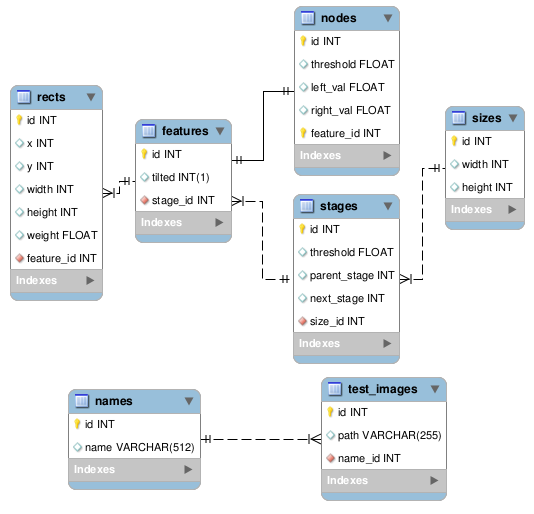
\includegraphics[width=\textwidth]{er_diagram.png}
    \caption{Схема базы данных}
    \label{fig:er_diagram}
\end{figure}

\subsubsection{Каскад Хаара}

В процессе работы приложения, алгоритм Виолы-Джонса использует стандартный каскад Хаара \cite{haar_cascade},
который был обучен ранее на большом объеме тестовых изображений.
Стандартный каскад представлен XML-документом и свободно доступен для загрузки.
Для более производительной работы приложения, каскад был перенесен из формата
XML в базу данных с помощью Perl-скрипта.

Приведем часть первого \textit{stage} из стандартного каскада:
\begin{verbatim}
<haarcascade_frontalface_alt>
  <size>20 20</size>
  <stages>
    <_>
      <!-- stage 0 -->
      <trees>
        <_>
          <!-- tree 0 -->
          <_> 
            <!-- root node -->
            <feature>
              <rects>
                <_>3 7 14 4 -1.</_>
                <_>3 9 14 2 2.</_></rects>
              <tilted>0</tilted></feature>
            <threshold>4.0141958743333817e-003</threshold>
            <left_val>0.0337941907346249</left_val>
            <right_val>0.8378106951713562</right_val></_></_>
        <_>
          <!-- tree 1 -->
          <_>
            <!-- root node -->
            <feature>
              <rects>
                <_>1 2 18 4 -1.</_>
                <_>7 2 6 4 3.</_></rects>
              <tilted>0</tilted></feature>
            <threshold>0.0151513395830989</threshold>
            <left_val>0.1514132022857666</left_val>
            <right_val>0.7488812208175659</right_val></_></_>
        ...
      # после всех признаков (деревьев) ...
      <stage_threshold>6.9566087722778320</stage_threshold>
      <parent>0</parent>
      <next>-1</next></_>
      ...
\end{verbatim}

Для хранения каскада Хаара в приложении были использованы следующие таблицы из
схемы, изображенной на рисунке \ref{fig:er_diagram}:

\begin{description}
    \item[rects] \hfill \\
        Таблица содержит массив прямоугольников, которые характеризуют
        конкретный признак. Так как каждый примитив Хаара представляет собой комбинацию из
        областей черного и белого цвета (рис. \ref{fig:haar}), при чем область черного цвета только одна,
        то для кодирования одного примитива достаточно следующих полей:
        \begin{description}
            \item[x] -- определяет горизонтальную координату темной части признака;
            \item[y] -- определяет вертикальную координату темной части признака;
            \item[width] -- определяет ширину темной части признака;
            \item[height] -- определяет высоту темной части признака.
        \end{description}
        Кроме того, при расчетах, используемых в алгоритме Виолы-Джонса используется
        вес каждого прямоугольного признака, который определен в поле \textbf{weight} таблицы.
        Каждый признак в каскаде Хаара может иметь более чем один примитив. Поэтому, в поле \textbf{feature\_id}
        для каждого примитива определено, к какому признаку он относится;
    \item[nodes] \hfill \\
        Таблица содержит список узлов каскада Хаара. Каждый узел характеризуется набором характеристик, среди
        которых выделяются:
        \begin{description}
            \item[threshold]~-- предельное значение, при преодолении которого узел можно считать отвергнутым;
            \item[left\_val]~-- значение, на которое будет увеличена характеристика признака в случае, если узел был отвергнут;
            \item[right\_val]~-- значение, на которое будет увеличена характеристика признака в случае, если узел был принят; 
            \item[feature\_id]~-- индекс признака, к которому относится данный узел.
        \end{description}
    \item[features] \hfill \\
        Таблица содержит список признаков, которыми оперирует алгоритм Виолы-Джонса.
        Каждый признак в общем случае может содержать только один узел, но при этом он содержит в себе
        множество примитивов. Каждый признак является частью одного этапа распознавания. При этом признаков в одном этапе
        может быть много. Идентификатор этапа хранится в поле \textbf{stage\_id}. Каждый признак кроме того может быть под
        наклоном. Этот факт кодируется в поле \textbf{tilted}. Так как в данном приложении используются только основные признаки
        Хаара, это поле всегда содержит 0. Однако, так как предполагается дальнейшая доработка программного продукта с
        добавлением дополнительных признаков, поле имеет место быть;
    \item[stages] \hfill \\
        Таблица содержит список этапов распознавания. Каждый этап состоит из набора признаков.
        В ходе алгоритма происходит накопление суммарных значений признаков на каждом этапе.
        В случае, если накопленное значение превысило значение \textbf{threshold}, этап отвергается и алгоритм
        переходит к следующему сканирующему окну. Для навигации по каскаду, используются поля
        \textbf{parent\_stage} и \textbf{next\_stage}. Кроме того, каждый этап ссылается на таблицу \textbf{sizes},
        определяя тем самым масштаб, который необходимо применить к сканируемому окну;
    \item[sizes] \hfill \\
        Таблица содержит список размеров примитивов. При этом в поле \textbf{width} определена ширина примитива, а в
        поле \textbf{height}~-- высота. Потенциально, алгоритм Виолы-Джонса способен работать с примитивами различного размера,
        повышая тем самым детализацию признаков. Однако, в текущей реализации программы используется лишь примитивы размера
        $20\times20$ точек и таблица была создана с целью увеличения функционала в будущем.
\end{description}

\subsubsection{Анализируемые объекты}

В ходе своей работы, программный продукт использует нейронную сеть для определения принадлежности анализируемого
изображения конкретной личности. Сами же личности должны быть сохранены в базе данных для последующего использования.

Именно эти данные хранит таблица \textbf{names}, при чем в поле \textbf{name} хранится полная информация о человеке.
Так как приложение не подразумевает, что для идентификации человека будет использовано именно его имя, то одного поля вполне
достаточно.

\subsubsection{Тестовые данные}

В ходе тестирования приложения был использован набор изображений из базы изображений под названием
\textit{Yale Face Database B} \cite{yale_face_database}. Она содержит более 16000 изображений 28ми человек в различных позах
и с различным углом наклона головы. Для хранения информации о местонахождении изображений на жестком диске
компьютера, на котором производится тестирование, используется таблица \textbf{test\_images}.

\subsection{Модульное тестирование}
Для разработанного программного обеспечения были написаны модульные тесты,
позволяющие проверить корректность ранее оттестированного кода при внесении
изменений. Пример прогонки модульных тестов показан на рисунке
\ref{fig:test}. Пример исходного кода модульных тестов представлен в приложенни
\ref{ap1}.

\begin{figure}[hbt]
  \centering
  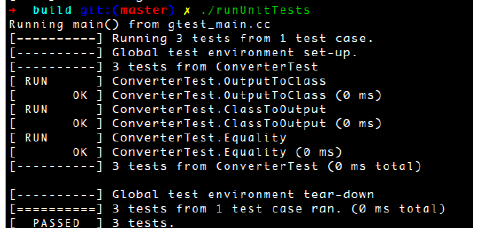
\includegraphics{tests.png}
  \caption{Пример прогона модульных тестов}
  \label{fig:test}
\end{figure}

\subsection{Структура программы}

Здесь мы опишем структуру программы, её основные элементы и устройство.
На рисунке \ref{fig:proj-struct} увидеть из каких модулей состоит программа.

\begin{figure}[h!]
  \centering
  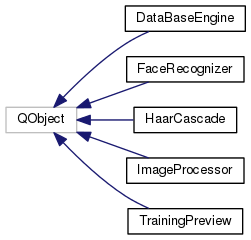
\includegraphics{uml.png}
  \caption{Структура программы}
  \label{fig:proj-struct}
\end{figure}

\subsection*{Выводы}
\addcontentsline{toc}{subsection}{Выводы}

Были рассмотрены основные методы, которые легли в основу разработанного
программного продукта. Была представлена и полностью описана схема базы данных,
была представлена диаграмма, показывающая структуру приложения.

\clearpage 
\section{Экспериментальный раздел}

В данном разделе будут представлены эксперименты, которые показывают
работоспособность созданного программного обеспечения.

\subsection{Достоверность распознавания}

Целью экспериментов является определение достоверности распознавания
разработанным программным продуктом. Достоверность распознавания определяется по
формуле
\[ \frac{TP}{TP+FP}, \]
где $TP$ - число правильно определенных объектов, $FP$ - число ложных обнаружений.


В эксперименте учавствуют 400 изображений, принадлежащие 40 людям.  Одно из
десяти изображений, принадлежащих одному человеку, является тестовым и не входит
в обучающую выборку.  В ходе экспериментов были получены результаты тестирования
скорости и достоверности распознавания. Результаты представлены на рисунке
\ref{fig:acc}.

\begin{figure}[h!]
  \centering
    \captionsetup{justification=centering}
  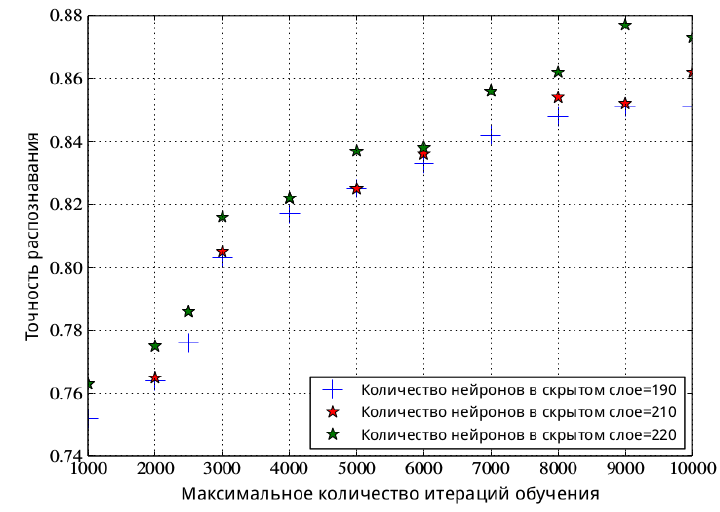
\includegraphics[width=.8\textwidth]{acc_from_iter.png}
  \caption{Исследование достоверности распознавания в зависимости от числа
максимальных итераций обучения нейронной сети.}
  \label{fig:acc}
\end{figure}

\subsection{Скорость распознавания}

Также были проведены исследования скорости обучения нейронной сети
в зависимости от максимального количества итераций. Результаты представлены на
рисунке \ref{fig:time}.

\begin{figure}[h!]
  \centering
    \captionsetup{justification=centering}
  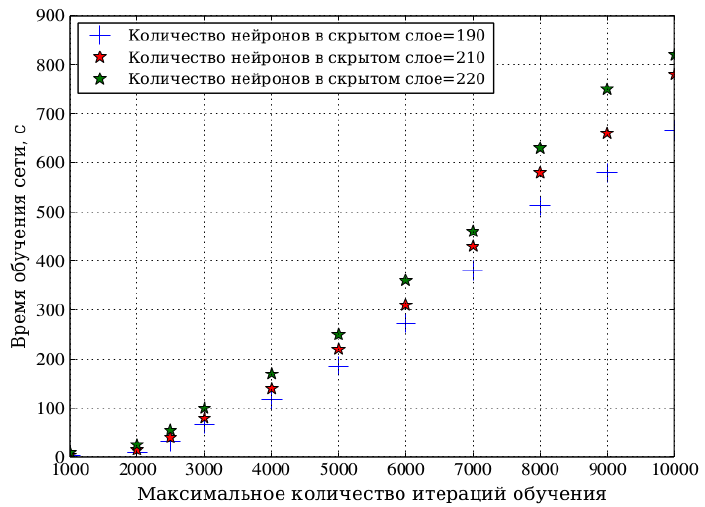
\includegraphics[width=.8\textwidth]{time_from_iter.png}
  \caption{Исследование времени обучения в зависимости от числа максимальных 
итераций обучения нейронной сети.}
  \label{fig:time}
\end{figure}

\subsection*{Выводы}
\addcontentsline{toc}{subsection}{Выводы}

Проведенные эксмперименты показали, что увеличение числа нейронов в сети
приводит к росту времени обучения нейронной сети, однако при большем числе нейронов в скрытом
слое, достоверность распознавания увеличивается.

\clearpage
